\section{Bozony i fermiony}
\subsection{Symetria}
\paragraph*{Równanie Schrödingera dla układu wielu cząstek}\mbox{}\\
%
\begin{equation*}
    i \hbar \dot{\Psi} = H \Psi
\end{equation*}
%
Z tego wynika: 
%
\begin{equation*}
    i \hbar \dot{\Psi}(q_1, \cdots, q_N, t) = H \Psi(q_1, \cdots, q_N, t)
\end{equation*}
%
gdzie $q_i$ to współrzędne położenia i pędu $i$-tej cząstki, N to liczba cząstek.
%
\\ \\
%
Wprowadzamy operator permutacji $P_{ij}$ dla $i$-tej i $j$-tej cząstki:
%
\begin{equation*}
    P_{ij} \Psi(q_1, \cdots, q_i, \cdots, q_j, \cdots, q_N, t) \equiv \Psi(q_1, \cdots, q_j, \cdots, q_i, \cdots, q_N, t)
\end{equation*}
%
Będziemy rozważać cząstki identyczne, czyli nierozróżnialne. Wtedy:
%
\begin{equation*}
    H(P_{ij}\Psi) = P_{ij} (H \Psi) \implies [H, P_{ij}] = 0
\end{equation*}
%
% Zatem operator $H$ jest symetryczny względem permutacji $P_{ij}$. % nie wiem co to niby miałoby znaczyć.
%
Operator $P_{ij}$ jest operatorem liniowym i $P_{ij}^2 = I$; w szczególności
jest unitarny. Ponieważ jest też Hermitowski, jego wartości własne to $\pm 1$.
%
\paragraph*{Funkcje falowe}\mbox{}\\
%
Skoro $H$ oraz $P_{ij}$ są Hermitowskie i komutują, możemy znaleźć wspólną bazę
funkcji własnych. Naturalnie dzielimy je na dwa typy --- związane z wartością
własną $1$ oraz z $-1$ dla operatora $P_{ij}$.
Dla układów identycznych cząstek
pierwszy typ nazywamy funkcjami symetrycznymi $\psi_+$:
%
\begin{equation*}
    \begin{aligned}
        P_{ij} \psi_+ (q_1, \cdots, q_i, \cdots, q_j, \cdots, q_N, t) &\equiv \psi_+ (q_1, \cdots, q_j, \cdots, q_i, \cdots, q_N, t) \\
        &\equiv \psi_+ (q_1, \cdots, q_i, \cdots, q_j, \cdots, q_N, t)
    \end{aligned}
\end{equation*}
%
Drugi typ --- funkcje antysymetryczne $\psi_-$, które zmieniają znak
pod działaniem operatora permutacji.
Oznacza to, że zamiana miejscami dwóch identycznych cząstek prowadzi
do zmiany znaku całej funkcji falowej:
%
\begin{equation*}
    P_{ij} \Psi_- (q_1, \cdots, q_i, \cdots, q_j, \cdots, q_N, t) = - \Psi_- (q_1, \cdots, q_i, \cdots, q_j, \cdots, q_N, t)
\end{equation*}
Ta antysymetryczna właściwość jest fundamentalna dla fermionów i prowadzi bezpośrednio do zasady wykluczenia Pauliego.
Funkcje antysymetryczne charakteryzują się tym, że prawdopodobieństwo
znalezienia dwóch fermionów w tej samej pozycji wynosi zero:
jeśli $q_i = q_j$, to zastosowanie permutacji z jednej strony zmienia
znak funkcji falowej, a z drugiej go zachowuje (permutacja identycznych
elementów to identyczność). Stąd wartość musi być zerowa.
Oznacza to, że fermiony ,,unikają'' siebie nawzajem.
%
\\ \\
%
Możemy rozważyć operator uogólniony $\hat{P}: P \Psi = P_{ij}P_{ik} \cdots \Psi$
%
\begin{equation*}
    P \Psi  (q_1, \cdots, q_n) = \Psi(q_{P_1}, \cdots, q_{P_n}).
\end{equation*}
%
Wtedy
\begin{equation*}
    P \psi_+ \equiv \psi_+
\end{equation*}
%
\begin{equation*}
    P \psi_- =
    \begin{cases}
        \psi_- & \text{dla parzystej permutacji} \\
        - \psi_- & \text{dla nieparzystej permutacji}
    \end{cases}
\end{equation*}
%
\paragraph*{Postulat}\mbox{}\\
%
Jeżeli spin jest połówkowy $s = \frac{n}{2}$, $n \in 2\mathbb{N} + 1$
--- układ identycznych cząstek znajduje się w antysymetrycznym stanie $\psi_-$,
to mówimy, że cząstki są \textbf{fermionami}.
Jeżeli spin jest całkowity $s = n$, $n \in \mathbb{N}$
--- układ identycznych cząstek znajduje się w symetrycznym stanie
$\psi_+$, to mówimy, że cząstkik są \textbf{bozonami}.
%
\paragraph*{Przykłady}\mbox{}\\
\begin{itemize}
    \item Elektron: $s = \frac{1}{2}$ --- fermion
    \item Proton: $s = \frac{1}{2}$ --- fermion
    \item atom: może być bozonem lub fermionem.
\end{itemize}
%
\subsection{Całkowicie symetryczne oraz całkowicie antysymetryczne \texorpdfstring{\\}{} funkcje falowe}
%
Będziemy rozważać teraz symetryzacje ($\Psi_s$) i antysymetryzacje ($\Psi_a$)
funkcji falowej dla N cząstek.
Dla $N = 2$ mamy:
%
\begin{equation*}
    \Psi_s (q_1, q_2) = \frac{1}{\sqrt{2}} \left( \Psi(q_1, q_2) + \Psi(q_2, q_1) \right)
\end{equation*}
%
\begin{equation*}
    \Psi_a (q_1, q_2) = \frac{1}{\sqrt{2}} \left( \Psi(q_1, q_2) - \Psi(q_2, q_1) \right)
\end{equation*}
%
Dla $N = 3$ mamy:
%
\begin{align*}
    \Psi_s (q_1, q_2, q_3) &= \frac{1}{\sqrt{6}} \big( 
        \Psi(q_1, q_2, q_3) + \Psi(q_1, q_3, q_2) + \Psi(q_2, q_1, q_3) \\
        &\quad + \Psi(q_2, q_3, q_1) + \Psi(q_3, q_1, q_2) + \Psi(q_3, q_2, q_1)
    \big)
\end{align*}
%
Ogólnie, jest to suma po wszystkich permutacjach trzech cząstek, znormalizowana
przez pierwiastek z liczby wszystkich permutacji --- wówczas prawdopodobieństwo
pozostaje jedynką.
%
Zakładamy brak oddziaływań między cząstkami, tzn. zapisujemy Hamiltonian w postaci:
%
\begin{equation*}
    H(q_1, \cdots, q_N) = h_1(q_1) \cdot h_2(q_2) \cdots h_N(q_N)
\end{equation*}
%
Wtedy możemy rozpisać Równanie Schrödingera:
%
\begin{equation*}
    h_i u_i = \epsilon_i u_i \quad \forall_{i = 1, 2, \ldots, N}
\end{equation*}
%
Dla $N = 2$ mamy i symetrycznej funkcji falowej mamy
\begin{equation*}
    \Psi_s(q_1, q_2) = \frac{1}{\sqrt{2}} (u_\alpha(q_1) u_\beta(q_2) + u_\beta(q_1) u_\alpha(q_2))
\end{equation*}
%
Dla antysymetrycznej funkcji falowej zmienia się znak:
%
\begin{equation*}
    \Psi_a(q_1, q_2) = \frac{1}{\sqrt{2}} (u_\alpha(q_1) u_\beta(q_2) - u_\beta(q_1) u_\alpha(q_2))
\end{equation*}
Zauważmy, że ta postać jest unormowanym wyznacznikiem
\begin{equation*}
    \begin{vmatrix}
        u_\alpha(q_1) & u_\beta(q_1) \\
        u_\alpha(q_2) & u_\beta(q_2)
    \end{vmatrix}.
\end{equation*}
%
$\Psi_a$ oraz $\Psi_s$ nie są prostymi iloczynami $u_\alpha$ i $u_\beta$.
Oznacza to, że są to stany splątane kwantowo ---
cząstki nie mogą być opisane niezależnie od siebie.
Dla uogólnionego przypadku $N = N$ (N cząstek) mamy:
%
\begin{equation*}
    \Psi_\triangle (q_1, \cdots, q_N) = \frac{1}{\sqrt{N!}}
    \begin{vmatrix}
        u_\alpha(q_1) & u_\beta(q_1) & \cdots & u_\nu(q_1) \\
        u_\alpha(q_2) & u_\beta(q_2) & \cdots & u_\nu(q_2) \\
        \vdots & \vdots & \ddots & \vdots \\
        u_\alpha(q_N) & u_\beta(q_N) & \cdots & u_\nu(q_N)
    \end{vmatrix}
\end{equation*}
%
Wyznacznik, który się pojawił jest wyznacznikiem Slatera.
%
Sumując powyższe wzory otrzymujemy:
%
\begin{equation*}
    \Psi_A (q_1, \cdots, q_N) = \frac{1}{\sqrt{N!}} \sum_{P} (-1)^{P} P u_\alpha(q_1) u_\beta(q_2) \cdots u_\nu(q_N)
\end{equation*}
%
\begin{equation*}
    \Psi_S (q_1, \cdots, q_N) = \frac{1}{\sqrt{N!}} \sum_{P} P u_\alpha(q_1) u_\beta(q_2) \cdots u_\nu(q_N)
\end{equation*}
%
\subsection{Zasada Pauliego}
%
Rozważamy antysymetryczny układ elektronów (fermiony). \textbf{Pytanie}: Co będzie, gdy $u_\alpha = u_\beta$?
%
Gdy $u_\alpha$ = $u_\beta$ to wyznacznik Slatera jest równy 0.
%
\begin{equation*}
    \Psi_A (q_1, \cdots, q_N) = 0
\end{equation*}
%
Zatem dwa elektrony nie mogą znajdować się w tym samym stanie.
%
\textbf{Zasada}: Tylko jeden fermion może okupować dany stan kwantowy.
%
\paragraph*{Przykład}\mbox{}\\
%
$l < n$, $l \in \mathbb{N}$, $-l \leq m \leq l$
%
\\ \\
%
Przykład diagramu energetycznego pokazującego różne stany kwantowe dla elektronów w atomie.
\begin{figure}[H]
    \centering
    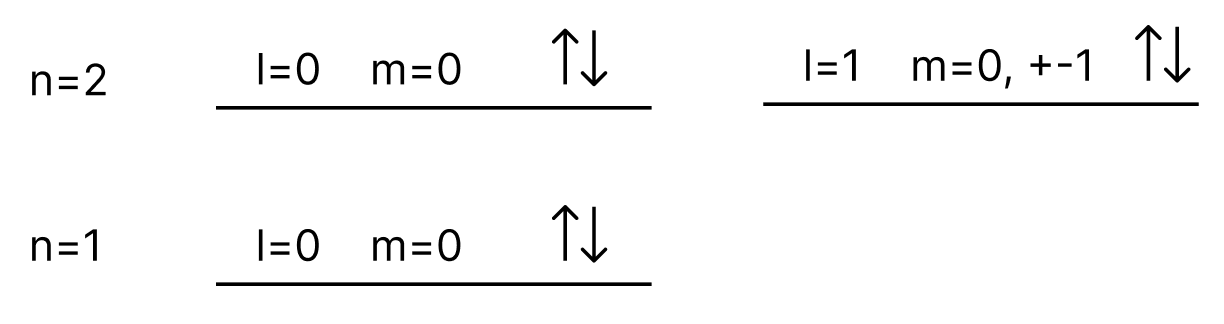
\includegraphics[width=0.5\textwidth]{bozony_fermiony}
    \label{fig:bozony_fermiony}
\end{figure}
\begin{equation*}
    N_e(1s^2, 2s^2, 2p^6)
\end{equation*}
Liczba w wykładniku to liczba elektronów w danym stanie (w danym orbitalu na danym poziomie). Zmienna $n$ numeruje poziomy energetyczne. Na pierwszym
poziomie występuje jeden orbital $1s$, na drugim poziomie występują dwa orbitale $2s$ i $2p$ - mieszczą odpowiednio 2, 2, 6 elektronów. Zmienna $l$ to
orbitalna liczba kwantowa - $0$ odpowiada orbitalowi $s$, $1$ odpowiada orbitalowi $p$, $2$ odpowiada orbitalowi $d$, $3$ odpowiada orbitalowi $f$.
Zmienna $m$ to magnetyczna liczba kwantowa - opisuje orientację orbitalu w przestrzeni. Orbital $s$ ma tylko jedną możliwą orientację,
stąd $m = 0$. Orbital $p$ ma trzy możliwe orientacje, stąd $m = -1, 0, 1$.
\paragraph*{Wniosek}\mbox{}\\
Bez tej zasady świat byłby inny, albo by nie istniał. Bez tej zasady wszystkie elektrony byłyby w tym samym stanie (skondensowałyby się w jednym stanie),
czyli w najniższym stanie energetycznym, co oznaczałoby brak różnorodności pierwiastków chemicznych i stabilnych struktur molekularnych.
%
Zasada Pauliego jest podstawową własnością cząstek.
%
\textbf{Pytanie}: Czym są strzałki góra/dół? Strzałka reprezentuje spin elektronu, który może mieć wartość $m_s = \pm \frac{1}{2}$ (magnetyczna liczba spinowa).
